\section{Edge-Hardware Validation}
\label{sec:edge_hardware}

Latency numbers in the stereo literature are overwhelmingly reported on desktop GPUs. Table~\ref{tab:efficient_comparison} catalogues the full distribution of reporting hardware for 41 representative methods: NVIDIA Titan X (3 methods), Titan V/Xp (3), GTX 1080Ti (6), Tesla V100 (5), RTX 2080Ti (3), RTX 3090 (12), and RTX 4090 (5). Only three methods in our survey report latency on actual embedded accelerators: AnyNet~\cite{wang2019anynet} on Jetson TX2, Pip-Stereo~\cite{zheng2026pipstereo} on Jetson Orin NX, and (in published artifacts but not the headline result) HITNet~\cite{tankovich2021hitnet} on a TPU-Edge variant.

The discrepancy is significant because the architectural decisions that drive desktop-GPU latency (large memory bandwidth, fast 3D-conv kernels, tolerance for control-flow overhead) often differ from those that drive edge-accelerator latency (limited memory, slower 3D-conv kernels, sensitivity to operator fusion). This section documents what is known about how the methods of Section~\ref{sec:taxonomy} actually perform on edge hardware. Fig.~\ref{fig:param_pareto} complements Fig.~\ref{fig:pareto_kitti} by showing the same methods under a different cost axis: parameter count rather than inference latency.

\begin{figure*}[!htbp]
\centering
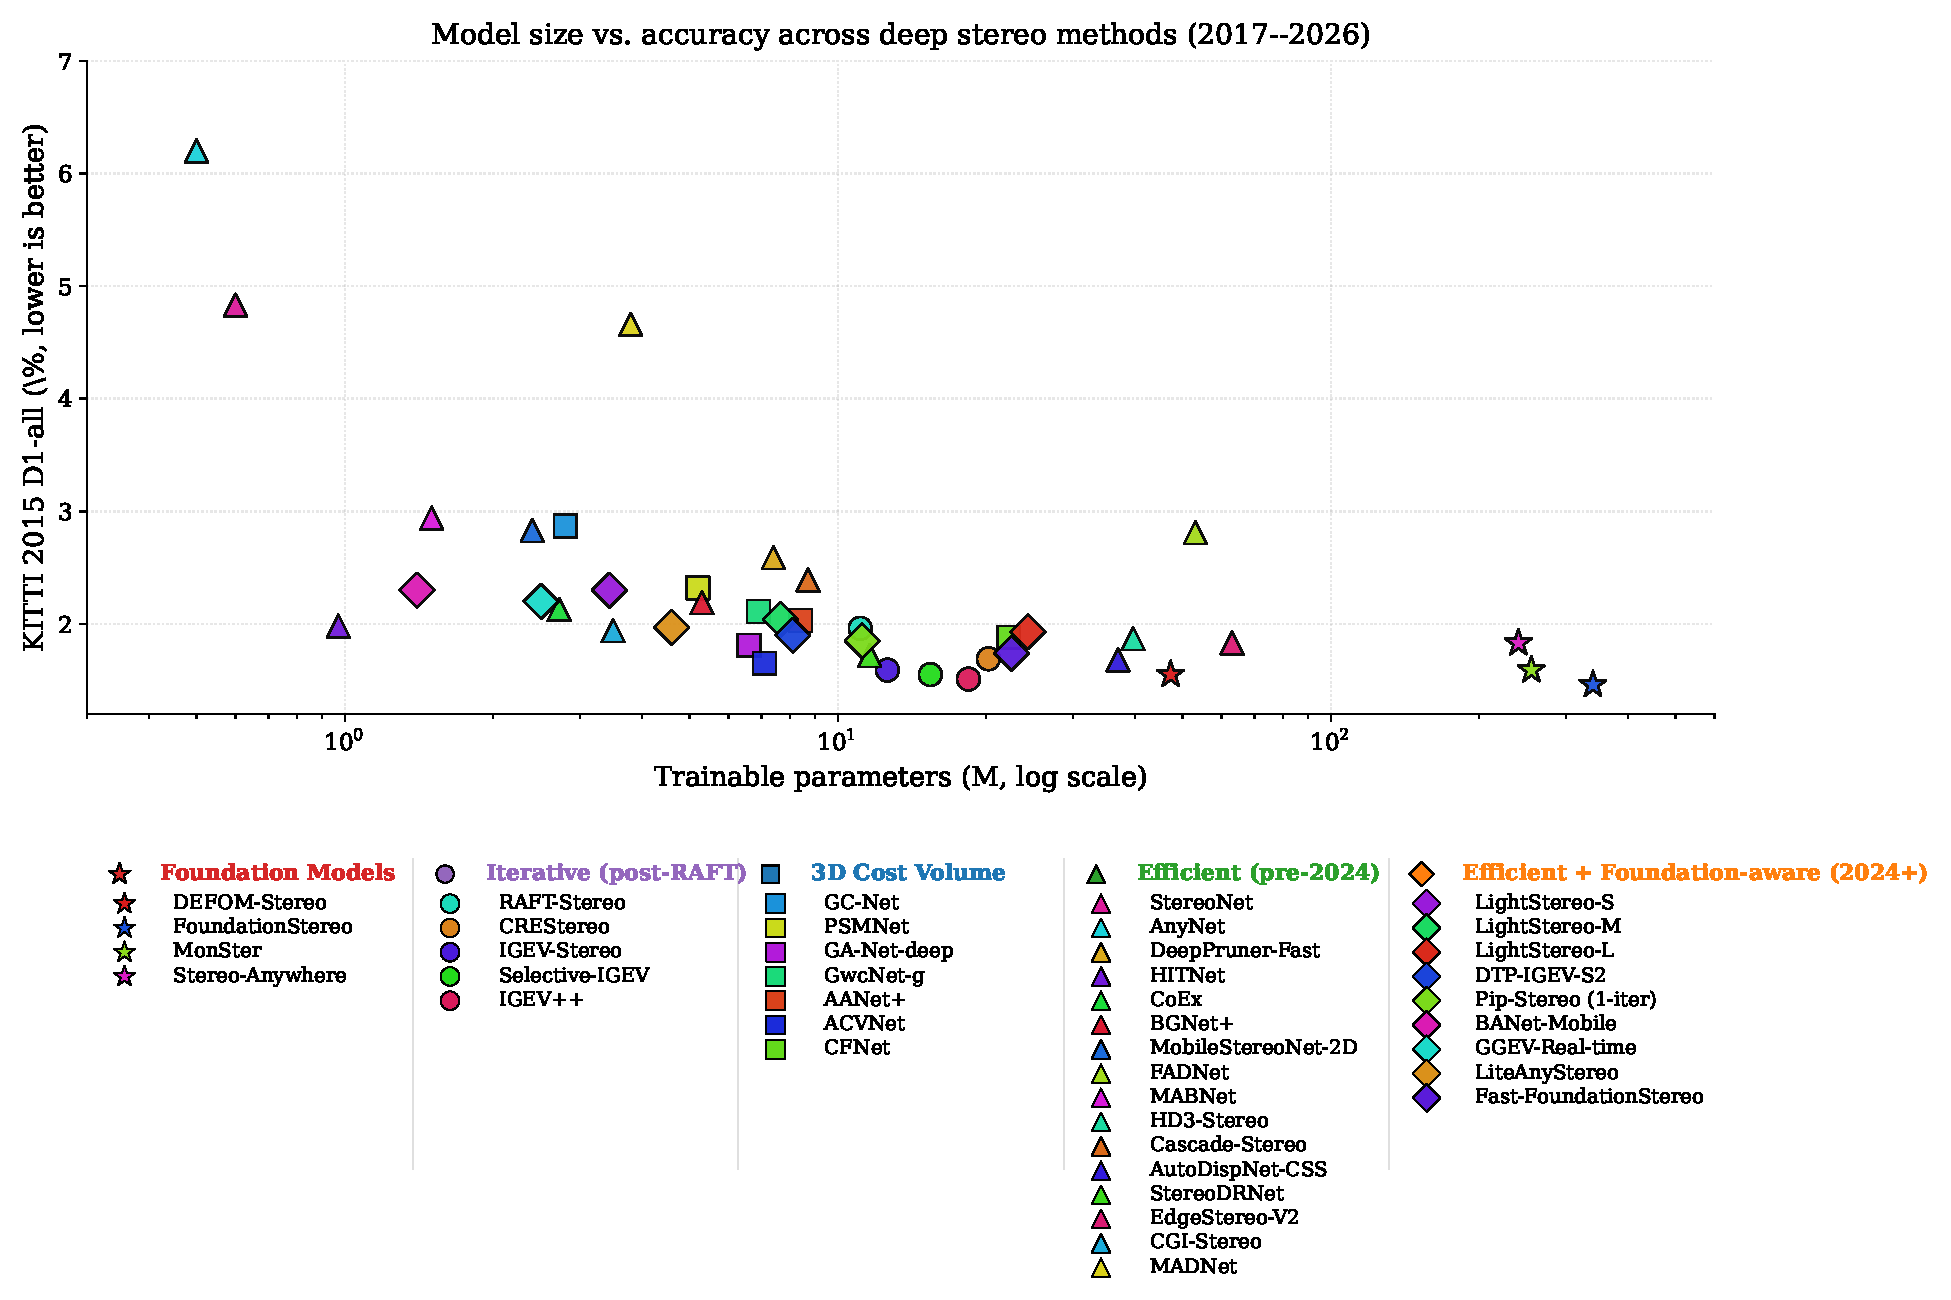
\includegraphics[width=0.95\textwidth]{figures/fig_param_pareto.pdf}
\caption{Model size versus accuracy across the surveyed methods. Markers and colours follow Fig.~\ref{fig:pareto_kitti}. The same data points as Fig.~\ref{fig:pareto_kitti} are shown but with parameter count on the horizontal axis instead of latency. Parameter count and latency are not strictly proportional: low-parameter methods are not always low-latency (e.g.\ MobileStereoNet-2D at 2.4\,M parameters but 380\,ms latency), and vice versa, because the two depend on different operator-level efficiencies.}
\label{fig:param_pareto}
\end{figure*}

\subsection{What Is an Edge Accelerator?}

For concreteness we distinguish three tiers of inference platform.

\textbf{Desktop GPU} (RTX 3090, RTX 4090): 24--80\,GB GDDR6X memory, 600--1000\,GB/s memory bandwidth, dedicated tensor cores, full FP32/FP16/BF16/INT8 support, hundreds of watts of thermal envelope. The standard reporting platform for the stereo literature.

\textbf{Datacenter GPU} (A100, H100): similar to desktop-GPU but with HBM memory and substantially higher bandwidth (1.5--3\,TB/s). The cost-per-deployment makes this tier impractical for most stereo applications; we mention it for completeness.

\textbf{Embedded accelerator}: NVIDIA Jetson family (Orin Nano, Orin NX, AGX Orin), Qualcomm RB5/RB6, Apple M1/M2 Neural Engine, and similar. These devices have 4--64\,GB unified memory, 65--200\,GB/s memory bandwidth, 5--60\,W thermal envelopes, and tend to be memory-bandwidth-bound rather than compute-bound for the operator mix typical of stereo networks. The Jetson Orin Nano (8\,GB unified, 67~GB/s, 7--15\,W) is the most common ``serious deployment but cost-sensitive'' target and is the implicit benchmark for several of the recent edge-stereo papers.

\subsection{Operators That Cost Differently on Edge}

Three operator classes have very different relative costs on edge versus desktop hardware.

\textbf{3D convolutions} are well-supported by desktop GPU tensor cores but poorly supported by most edge accelerators, where they fall back to slower general-purpose paths. This is a major reason the architectural-compression family of Section~\ref{ssec:arch} (BANet~\cite{xu2025banet}, LightStereo~\cite{guo2025lightstereo}) deliberately replaces 3D convolutions with 2D operations.

\textbf{Iterative loops with shared weights} (i.e., the GRU update of RAFT-Stereo and successors) impose control-flow overhead and break operator-fusion patterns that compilers like TensorRT rely on for desktop performance. Pip-Stereo~\cite{zheng2026pipstereo} reports that the per-iteration overhead on Jetson Orin NX is approximately 2--3$\times$ higher than on a desktop GPU of comparable peak FLOPs, which is one of the original motivations for iterative-loop compression (Section~\ref{ssec:iterloop}).

\textbf{Vision Transformers (ViT)} are supported on edge but poorly. The Depth Anything V2 ViT-Large used by DEFOM-Stereo~\cite{jiang2025defom}, FoundationStereo~\cite{wen2025foundationstereo}, and MonSter~\cite{cheng2025monster} cannot fit in the 8\,GB memory of a Jetson Orin Nano at FP16, even before any stereo branch. EfficientViT and RepViT are explicitly designed to address this, and Pip-Stereo's MPT~\cite{zheng2026pipstereo} and Fast-FoundationStereo~\cite{wen2026fastfoundationstereo} both use NAS-discovered Repuneted ViT variants in their student backbones.

\subsection{Reported Edge-Hardware Numbers}

The published edge numbers, while sparse, point in a consistent direction.

\textbf{AnyNet}~\cite{wang2019anynet}, evaluated on Jetson TX2 in 2019, was the first stereo network designed explicitly for edge deployment. AnyNet's four-stage anytime structure (Section~\ref{ssec:adaptive}) reports 12\,ms (stage 1) to 40\,ms (stage 4) on TX2 at the cost of 6.20\% to $\sim$4\% KITTI D1 respectively. By the standards of the time these were strong numbers; by 2026 they are below the accuracy floor of any practical deployment.

\textbf{HITNet}~\cite{tankovich2021hitnet} reports 18\,ms on a desktop Titan V at 1.98\% KITTI D1, but its tile-based architecture is one of the few that ports cleanly to TPU-class edge accelerators. Pip-Stereo's cross-domain analysis~\cite{zheng2026pipstereo} cites HITNet as a cautionary example: its single-pass design lacks the iterative refinement that protects cross-domain accuracy.

\textbf{Pip-Stereo}~\cite{zheng2026pipstereo} is the most recent and the most carefully validated edge-stereo paper at the time of writing. It reports 17\,ms on Jetson Orin NX at $480 \times 640$ resolution, at 1.85\% KITTI D1 (Pip-Stereo's 1-iteration variant). The reference comparison is DEFOM-Stereo on the same Orin NX, which the authors measure at 196\,ms (an 11.5$\times$ slowdown relative to Pip-Stereo). To our knowledge this is the only published direct comparison of a foundation-era and a compressed model on the same edge accelerator.

\textbf{Fast-FoundationStereo}~\cite{wen2026fastfoundationstereo} reports 85\,ms on a desktop RTX 4090 but does not include edge-accelerator numbers. The authors note that the EfficientViT student would fit in 4\,GB at FP16, suggesting that an Orin Nano deployment is plausible, but the actual measurement is not reported.

\subsection{Why More Edge Numbers Are Not Reported}

Several reasons explain the sparsity of edge-hardware reporting in the published literature:

\begin{itemize}
\item \textbf{Reviewer expectations}: top-tier vision conferences (CVPR, ICCV, NeurIPS) primarily reward top-of-leaderboard accuracy, which is reported on desktop GPUs. An edge-only result is often considered a separate paper rather than a primary contribution.
\item \textbf{Heterogeneity of edge hardware}: there is no single ``edge GPU'' analog to the RTX 3090. Jetson Orin Nano, Orin NX, Orin AGX, Qualcomm RB5, and Apple Neural Engine all differ substantially in memory bandwidth and operator support, and cross-platform comparison is unreliable.
\item \textbf{Tooling friction}: deploying a PyTorch model on an edge accelerator typically requires ONNX export, TensorRT (or platform-specific) compilation, INT8 calibration, and operator-fusion tuning. Each step introduces accuracy degradation that is not predictable from the desktop result.
\end{itemize}

The first item is gradually changing: ICRA, IROS, RAS and similar venues explicitly value embedded validation, and the 2024--2026 wave of edge-stereo papers (DTP at ICRA 2024~\cite{pan2024dtp}, LightStereo at ICRA 2025~\cite{guo2025lightstereo}, Pip-Stereo at CVPR 2026~\cite{zheng2026pipstereo}) has been increasingly explicit about edge-hardware validation.

\subsection{A Plea for Standardized Edge Reporting}

Only a few of the surveyed papers report a common subset of numbers. Pip-Stereo~\cite{zheng2026pipstereo} is the most complete: it reports latency on both an embedded accelerator (Jetson Orin NX) and a desktop GPU, accuracy on KITTI 2015, Middlebury, ETH3D, and DrivingStereo weather subsets, and comparisons against foundation-model baselines on the same hardware. Most other efficient-stereo papers omit at least one of these axes. A standardised reporting protocol, covering embedded-accelerator latency, desktop-GPU latency, and zero-shot accuracy on the four standard cross-domain benchmarks, would make the cross-paper comparison in Table~\ref{tab:efficient_comparison} considerably less noisy; we observe this without prescribing any specific protocol.
